%%% ---------- Figure A: the problem ----------
\newcommand{\figProblem}{%
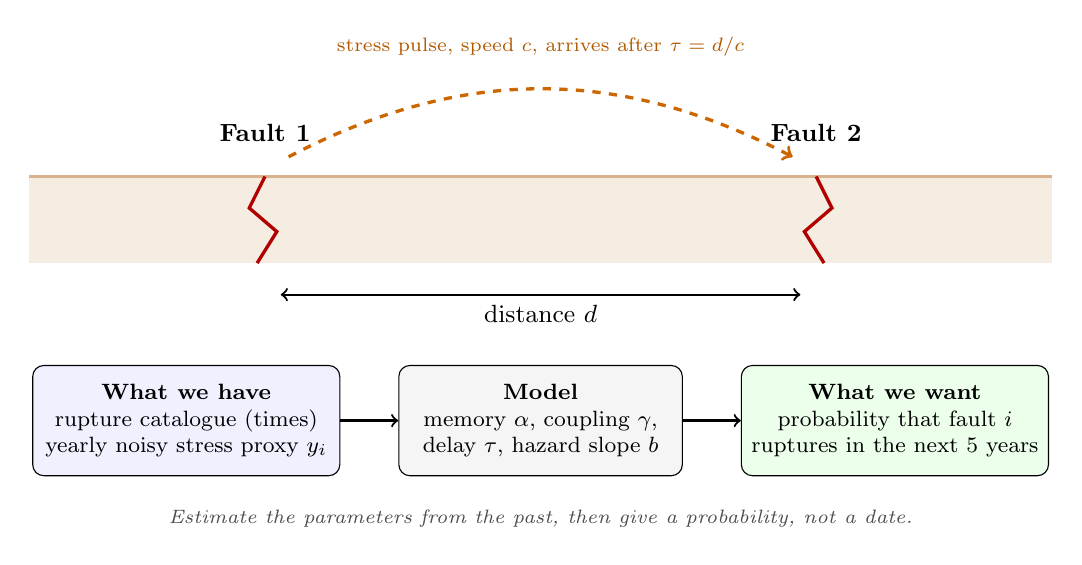
\begin{tikzpicture}[x=1cm,y=1cm,
  lab/.style={font=\small,align=center},
  bx/.style={font=\footnotesize,align=center,draw,rounded corners,minimum height=1.4cm},
  note/.style={font=\scriptsize,align=center,text=black!70}]
  % ground
  \fill[brown!15] (0,0) rectangle (13,-1.1);
  \draw[brown!60,thick] (0,0)--(13,0);
  % fault 1 and 2 (zig-zag lines going down)
  \draw[red!70!black,very thick] (3,0)--(2.8,-0.4)--(3.15,-0.7)--(2.9,-1.1);
  \draw[red!70!black,very thick] (10,0)--(10.2,-0.4)--(9.85,-0.7)--(10.1,-1.1);
  \node[lab] at (3,0.55) {\textbf{Fault 1}};
  \node[lab] at (10,0.55) {\textbf{Fault 2}};
  % distance
  \draw[<->,thick] (3.2,-1.5)--node[below,lab]{distance $d$}(9.8,-1.5);
  % pulse
  \draw[->,orange!80!black,very thick,dashed] (3.3,0.25) .. controls (5.5,1.4) and (7.5,1.4) .. (9.7,0.25);
  \node[note,orange!70!black] at (6.5,1.65) {stress pulse, speed $c$, arrives after $\tau=d/c$};
  % what we see
  \node[bx,fill=blue!6,minimum width=3.9cm] (obs) at (2.0,-3.1)
     {\textbf{What we have}\\ rupture catalogue (times)\\ yearly noisy stress proxy $y_i$};
  \node[bx,fill=gray!8,minimum width=3.6cm] (mod) at (6.5,-3.1)
     {\textbf{Model}\\ memory $\alpha$, coupling $\gamma$,\\ delay $\tau$, hazard slope $b$};
  \node[bx,fill=green!8,minimum width=3.9cm] (q) at (11.0,-3.1)
     {\textbf{What we want}\\ probability that fault $i$\\ ruptures in the next 5 years};
  \draw[->,thick] (obs)--(mod);
  \draw[->,thick] (mod)--(q);
  \node[note] at (6.5,-4.35) {\emph{Estimate the parameters from the past, then give a probability, not a date.}};
\end{tikzpicture}}

%%% ---------- Figure B: stress cycle, memory, hazard ----------
\newcommand{\figCycle}{%
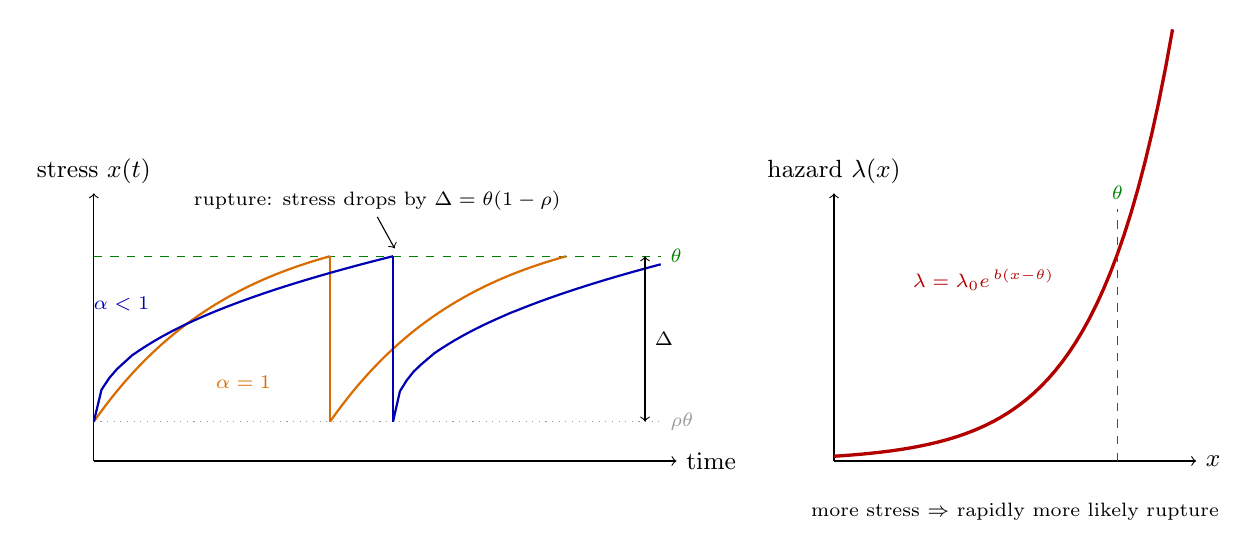
\begin{tikzpicture}[x=1.0cm,y=1.0cm,font=\small]
  % --- left: stress cycles
  \draw[->] (0,0)--(7.4,0) node[right]{time};
  \draw[->] (0,0)--(0,3.4) node[above]{stress $x(t)$};
  \draw[green!50!black,dashed] (0,2.6)--(7.2,2.6) node[right,font=\scriptsize]{$\theta$};
  \draw[black!40,dotted] (0,0.5)--(7.2,0.5) node[right,font=\scriptsize]{$\rho\theta$};
  % no memory (alpha=1): classical saturating curve, two cycles
  \draw[thick,orange!85!black] plot[domain=0:3,samples=40] (\x,{0.5+2.1*(1-exp(-0.55*\x))/(1-exp(-0.55*3))});
  \draw[thick,orange!85!black] (3,2.6)--(3,0.5);
  \draw[thick,orange!85!black] plot[domain=0:3,samples=40] ({3+\x},{0.5+2.1*(1-exp(-0.55*\x))/(1-exp(-0.55*3))});
  % with memory: fast start, slow end (power law)
  \draw[thick,blue!70!black] plot[domain=0:3.8,samples=40] (\x,{0.5+2.1*(\x/3.8)^0.45});
  \draw[thick,blue!70!black] (3.8,2.6)--(3.8,0.5);
  \draw[thick,blue!70!black] plot[domain=0:3.4,samples=40] ({3.8+\x},{0.5+2.1*(\x/3.8)^0.45});
  % drop
  \draw[<->] (7.0,0.5)--node[right,font=\scriptsize]{$\Delta$}(7.0,2.6);
  \node[font=\scriptsize,orange!85!black] at (1.9,1.0) {$\alpha=1$};
  \node[font=\scriptsize,blue!70!black] at (0.35,2.0) {$\alpha<1$};
  \node[font=\scriptsize,align=center] at (3.6,3.3) {rupture: stress drops by $\Delta=\theta(1-\rho)$};
  \draw[->,font=\scriptsize] (3.6,3.1)--(3.82,2.7);
  % --- right: hazard
  \begin{scope}[xshift=9.4cm]
    \draw[->] (0,0)--(4.6,0) node[right]{$x$};
    \draw[->] (0,0)--(0,3.4) node[above]{hazard $\lambda(x)$};
    \draw[very thick,red!70!black] plot[domain=0:4.3,samples=50] (\x,{0.06*exp(1.05*\x)});
    \draw[green!50!black,dashed] (3.6,0)--(3.6,3.2) node[above,font=\scriptsize]{$\theta$};
    \node[font=\scriptsize,red!70!black,align=center] at (1.9,2.3) {$\lambda=\lambda_0e^{\,b(x-\theta)}$};
    \node[font=\scriptsize,align=center] at (2.3,-0.65) {more stress $\Rightarrow$ rapidly more likely rupture};
  \end{scope}
\end{tikzpicture}}

%%% ---------- Figure C: delayed pulse timeline ----------
\newcommand{\figDelay}{%
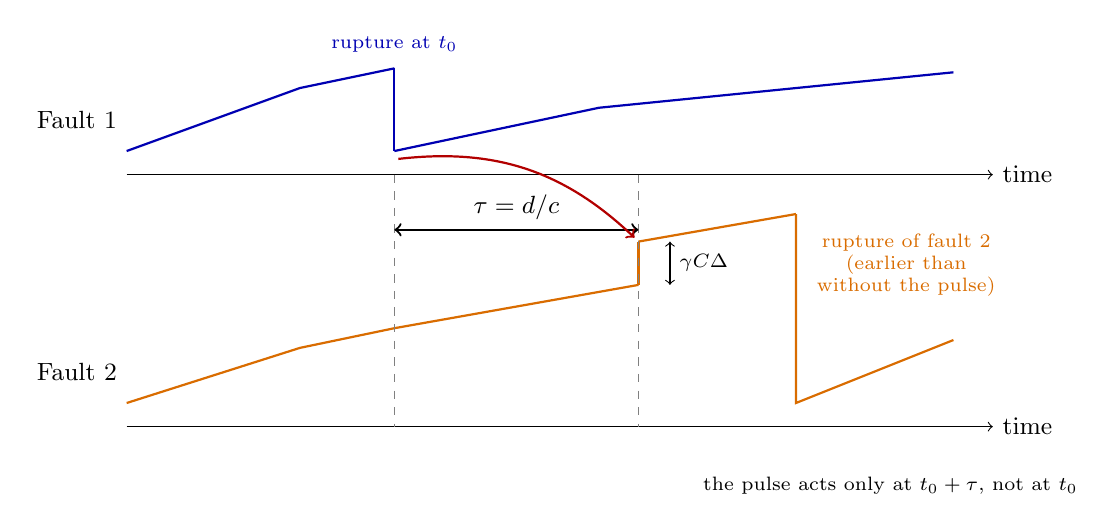
\begin{tikzpicture}[x=1cm,y=1cm,font=\small]
  % fault 1 axis
  \draw[->] (0,3.6)--(11,3.6) node[right]{time};
  \node[left] at (0,4.3) {Fault 1};
  \draw[blue!70!black,thick] (0,3.9)--(2.2,4.7)--(3.4,4.95);
  \draw[blue!70!black,thick] (3.4,4.95)--(3.4,3.9);
  \draw[blue!70!black,thick] (3.4,3.9)--(6,4.45)--(10.5,4.9);
  \node[blue!70!black,font=\scriptsize] at (3.4,5.25) {rupture at $t_0$};
  % fault 2 axis
  \draw[->] (0,0.4)--(11,0.4) node[right]{time};
  \node[left] at (0,1.1) {Fault 2};
  \draw[orange!85!black,thick] (0,0.7)--(2.2,1.4)--(3.4,1.65)--(6.5,2.2);
  \draw[orange!85!black,thick] (6.5,2.2)--(6.5,2.75);       % jump gamma*C*Delta
  \draw[orange!85!black,thick] (6.5,2.75)--(8.5,3.1);
  \draw[orange!85!black,thick] (8.5,3.1)--(8.5,0.7)--(10.5,1.5);
  \node[orange!85!black,font=\scriptsize,align=center] at (9.9,2.45) {rupture of fault 2\\ (earlier than\\ without the pulse)};
  % delay arrows
  \draw[dashed,gray] (3.4,3.6)--(3.4,0.4);
  \draw[dashed,gray] (6.5,3.6)--(6.5,0.4);
  \draw[<->,thick] (3.4,2.9)--node[above]{$\tau=d/c$}(6.5,2.9);
  \draw[->,red!70!black,thick] (3.45,3.8) to[bend left=25] (6.45,2.8);
  \node[red!70!black,font=\scriptsize] at (4.4,3.4) {};
  \draw[<->] (6.9,2.2)--node[right,font=\scriptsize]{$\gamma C\Delta$}(6.9,2.75);
  \node[font=\scriptsize,align=center] at (9.7,-0.35) {the pulse acts only at $t_0+\tau$, not at $t_0$};
\end{tikzpicture}}

%%% ---------- Figure D: inference pipeline ----------
\newcommand{\figPipeline}{%
\begin{tikzpicture}[node distance=0.55cm and 0.7cm,
  box/.style={draw,rounded corners=2pt,align=center,minimum height=1.05cm,minimum width=2.5cm,font=\small,fill=gray!7},
  hi/.style={box,fill=blue!8},
  outb/.style={box,fill=green!9},
  arr/.style={-{Latex[length=2mm]},thick}]
  \node[box] (par) {parameters\\ $\vartheta=(\alpha,\gamma,c,b)$};
  \node[box,right=of par] (soe) {memory $\to$ sum of\\ exponentials (Markov)};
  \node[hi,right=of soe] (pf) {particle filter\\ $\hat\ell(\vartheta)$};
  \node[box,right=of pf] (opt) {Nelder--Mead\\ $\hat\vartheta=\arg\max\hat\ell$};
  \node[box,below=0.9cm of par] (dat) {data: catalogue\\ + yearly $y_i$};
  \node[outb,below=0.9cm of soe] (lr) {LR tests\\ $\alpha=1$, $\gamma=0$\\ (bootstrap)};
  \node[outb,below=0.9cm of pf] (prof) {profile\\ likelihood};
  \node[outb,below=0.9cm of opt] (fc) {$P(\text{rupture in }(t,t+W])$\\ vs.\ Poisson, Weibull};
  \draw[arr] (par)--(soe); \draw[arr] (soe)--(pf); \draw[arr] (pf)--(opt);
  \draw[arr] (dat)--(par); 
  \draw[arr] (opt)--(fc); \draw[arr] (pf)--(prof); \draw[arr] (opt.south west)--(lr.north east);
  \draw[arr,dashed] (opt.north) -- ++(0,0.55) -| (par.north);
\end{tikzpicture}}
